\documentclass[12pt,ignorenonframetext,compress]{beamer}
\setbeamertemplate{caption}[numbered]
\setbeamertemplate{caption label separator}{: }
\setbeamercolor{caption name}{fg=normal text.fg}
\beamertemplatenavigationsymbolsempty
\usepackage{lmodern}
\usepackage{amssymb,amsmath}
\usepackage{ifxetex,ifluatex}
\usepackage{fixltx2e} % provides \textsubscript
\ifnum 0\ifxetex 1\fi\ifluatex 1\fi=0 % if pdftex
  \usepackage[T1]{fontenc}
  \usepackage[utf8]{inputenc}
\else % if luatex or xelatex
  \ifxetex
    \usepackage{mathspec}
  \else
    \usepackage{fontspec}
  \fi
  \defaultfontfeatures{Ligatures=TeX,Scale=MatchLowercase}
\fi
\usetheme[]{metropolis}
% use upquote if available, for straight quotes in verbatim environments
\IfFileExists{upquote.sty}{\usepackage{upquote}}{}
% use microtype if available
\IfFileExists{microtype.sty}{%
\usepackage{microtype}
\UseMicrotypeSet[protrusion]{basicmath} % disable protrusion for tt fonts
}{}
\newif\ifbibliography
\hypersetup{
            pdftitle={Week 4: Discrete Random Variables and Probability Distributions},
            pdfauthor={Sahir Bhatnagar},
            pdfborder={0 0 0},
            breaklinks=true}
\urlstyle{same}  % don't use monospace font for urls
\usepackage{color}
\usepackage{fancyvrb}
\newcommand{\VerbBar}{|}
\newcommand{\VERB}{\Verb[commandchars=\\\{\}]}
\DefineVerbatimEnvironment{Highlighting}{Verbatim}{commandchars=\\\{\}}
% Add ',fontsize=\small' for more characters per line
\usepackage{framed}
\definecolor{shadecolor}{RGB}{248,248,248}
\newenvironment{Shaded}{\begin{snugshade}}{\end{snugshade}}
\newcommand{\KeywordTok}[1]{\textcolor[rgb]{0.13,0.29,0.53}{\textbf{#1}}}
\newcommand{\DataTypeTok}[1]{\textcolor[rgb]{0.13,0.29,0.53}{#1}}
\newcommand{\DecValTok}[1]{\textcolor[rgb]{0.00,0.00,0.81}{#1}}
\newcommand{\BaseNTok}[1]{\textcolor[rgb]{0.00,0.00,0.81}{#1}}
\newcommand{\FloatTok}[1]{\textcolor[rgb]{0.00,0.00,0.81}{#1}}
\newcommand{\ConstantTok}[1]{\textcolor[rgb]{0.00,0.00,0.00}{#1}}
\newcommand{\CharTok}[1]{\textcolor[rgb]{0.31,0.60,0.02}{#1}}
\newcommand{\SpecialCharTok}[1]{\textcolor[rgb]{0.00,0.00,0.00}{#1}}
\newcommand{\StringTok}[1]{\textcolor[rgb]{0.31,0.60,0.02}{#1}}
\newcommand{\VerbatimStringTok}[1]{\textcolor[rgb]{0.31,0.60,0.02}{#1}}
\newcommand{\SpecialStringTok}[1]{\textcolor[rgb]{0.31,0.60,0.02}{#1}}
\newcommand{\ImportTok}[1]{#1}
\newcommand{\CommentTok}[1]{\textcolor[rgb]{0.56,0.35,0.01}{\textit{#1}}}
\newcommand{\DocumentationTok}[1]{\textcolor[rgb]{0.56,0.35,0.01}{\textbf{\textit{#1}}}}
\newcommand{\AnnotationTok}[1]{\textcolor[rgb]{0.56,0.35,0.01}{\textbf{\textit{#1}}}}
\newcommand{\CommentVarTok}[1]{\textcolor[rgb]{0.56,0.35,0.01}{\textbf{\textit{#1}}}}
\newcommand{\OtherTok}[1]{\textcolor[rgb]{0.56,0.35,0.01}{#1}}
\newcommand{\FunctionTok}[1]{\textcolor[rgb]{0.00,0.00,0.00}{#1}}
\newcommand{\VariableTok}[1]{\textcolor[rgb]{0.00,0.00,0.00}{#1}}
\newcommand{\ControlFlowTok}[1]{\textcolor[rgb]{0.13,0.29,0.53}{\textbf{#1}}}
\newcommand{\OperatorTok}[1]{\textcolor[rgb]{0.81,0.36,0.00}{\textbf{#1}}}
\newcommand{\BuiltInTok}[1]{#1}
\newcommand{\ExtensionTok}[1]{#1}
\newcommand{\PreprocessorTok}[1]{\textcolor[rgb]{0.56,0.35,0.01}{\textit{#1}}}
\newcommand{\AttributeTok}[1]{\textcolor[rgb]{0.77,0.63,0.00}{#1}}
\newcommand{\RegionMarkerTok}[1]{#1}
\newcommand{\InformationTok}[1]{\textcolor[rgb]{0.56,0.35,0.01}{\textbf{\textit{#1}}}}
\newcommand{\WarningTok}[1]{\textcolor[rgb]{0.56,0.35,0.01}{\textbf{\textit{#1}}}}
\newcommand{\AlertTok}[1]{\textcolor[rgb]{0.94,0.16,0.16}{#1}}
\newcommand{\ErrorTok}[1]{\textcolor[rgb]{0.64,0.00,0.00}{\textbf{#1}}}
\newcommand{\NormalTok}[1]{#1}
\usepackage{graphicx,grffile}
\makeatletter
\def\maxwidth{\ifdim\Gin@nat@width>\linewidth\linewidth\else\Gin@nat@width\fi}
\def\maxheight{\ifdim\Gin@nat@height>\textheight0.8\textheight\else\Gin@nat@height\fi}
\makeatother
% Scale images if necessary, so that they will not overflow the page
% margins by default, and it is still possible to overwrite the defaults
% using explicit options in \includegraphics[width, height, ...]{}
\setkeys{Gin}{width=\maxwidth,height=\maxheight,keepaspectratio}

% Prevent slide breaks in the middle of a paragraph:
\widowpenalties 1 10000
\raggedbottom

\AtBeginPart{
  \let\insertpartnumber\relax
  \let\partname\relax
  \frame{\partpage}
}
\AtBeginSection{
  \ifbibliography
  \else
    \let\insertsectionnumber\relax
    \let\sectionname\relax
    \frame{\sectionpage}
  \fi
}
\AtBeginSubsection{
  \let\insertsubsectionnumber\relax
  \let\subsectionname\relax
  \frame{\subsectionpage}
}

\setlength{\parindent}{0pt}
\setlength{\parskip}{6pt plus 2pt minus 1pt}
\setlength{\emergencystretch}{3em}  % prevent overfull lines
\providecommand{\tightlist}{%
  \setlength{\itemsep}{0pt}\setlength{\parskip}{0pt}}
\setcounter{secnumdepth}{0}
%% header.tex
%%
%% Copyright (C) 2016 - 2017  Dirk Eddelbuettel
%%
%% This file is part of samples-rmarkdown-metropolis repository.
%%
%% samples-rmarkdown-metropolis is free software: you can redistribute it
%% and/or modify it under the terms of the GNU General Public License as
%% published by the Free Software Foundation, either version 2 of the
%% License, or (at your option) any later version.
%%
%% samples-rmarkdown-metropolis is distributed in the hope that it will be
%% useful, but WITHOUT ANY WARRANTY; without even the implied warranty of
%% MERCHANTABILITY or FITNESS FOR A PARTICULAR PURPOSE.  See the GNU General
%% Public License for more details.
%%
%% You should have received a copy of the GNU General Public License along with
%% samples-rmarkdown-metropolis.  If not, see <http://www.gnu.org/licenses/>.

%% If you have the Fira font installed, to actually have it used it 
%% via rmarkdown you need to declare it here 
%\setsansfont[ItalicFont={Fira Sans Light Italic},BoldFont={Fira Sans},BoldItalicFont={Fira Sans Italic}]{Fira Sans Light}
%\setmonofont[BoldFont={Fira Mono Medium}]{Fira Mono}

%% You can set various Metropolis options via \metroset{} here
%\metroset{....}

%% You can redefine colours, mostly by borrowing from Beamer
\setbeamercolor{frametitle}{bg=gray}
\usepackage{graphicx}
%\graphicspath{ {/home/sahir/git_repositories/math697/images/} }
\usepackage{hyperref, url}
\usepackage{caption}
\usepackage[round,sort]{natbib}   % bibliography omit 'round' option if you prefer square brackets
\usepackage{float}
\usepackage{color, colortbl, xcolor}
\definecolor{lightgray}{RGB}{200,200,200}
\usepackage{array}
\newcolumntype{L}{>{\centering\arraybackslash}m{3cm}} % used for text wrapping in ctable
\usepackage{ctable}
\usepackage{nicefrac}
%\usepackage{calrsfs}
%\DeclareMathAlphabet{\pazocal}{OMS}{zplm}{m}{n}
%\newcommand{\La}{\mathcal{L}}
%\newcommand{\Lb}{\pazocal{L}}
\usepackage{pifont}% http://ctan.org/pkg/pifont
\newcommand{\cmark}{\ding{51}}%
\newcommand{\xmark}{\ding{55}}%
\def\widebar#1{\overline{#1}}

\def\Xmean{\skew3\widebar{X}}
\def\Ymean{\widebar{Y}}
\def\xmean{\bar{x}}
\def\ymean{\bar{y}}
\def\dint{\displaystyle\int}
\def\dsum{\displaystyle\sum}

\newcommand{\xbar}{\bar{x}}
\newcommand{\Xbar}{\bar{X}}
\newcommand{\sumn}{\dsum_{i=1}^{n}}

\metroset{numbering=fraction, block = fill}

%% change fontsize of R code
\let\oldShaded\Shaded
\let\endoldShaded\endShaded
\renewenvironment{Shaded}{\scriptsize\oldShaded}{\endoldShaded}

%% change fontsize of output
\let\oldverbatim\verbatim
\let\endoldverbatim\endverbatim
\renewenvironment{verbatim}{\scriptsize\oldverbatim}{\endoldverbatim}

\newtheorem{proposition}[theorem]{Proposition}
\newtheorem{exercise}[theorem]{Exercise}


%% You also use hyperref, and pick colors 
\hypersetup{colorlinks,citecolor=orange,filecolor=red,linkcolor=brown,urlcolor=blue}

\newcommand {\framedgraphiccaption}[2] {
            \begin{figure}
            \centering
            \includegraphics[width=\textwidth,height=0.8\textheight,keepaspectratio]{#1}
            \caption{#2}
            \end{figure}
}

\newcommand {\framedgraphic}[1] {
            \begin{figure}
            \centering
            \includegraphics[width=\textwidth,height=0.7\textheight,keepaspectratio]{#1}
            \end{figure}
}

%\usepackage{amsthm}
\setbeamertemplate{theorems}[numbered]

%% when rendered with rmarkdown, somehow the unicode char for the dot
%% disappears so we redefine it here -- that is an older comments, seems font-specific
%\renewcommand{\textbullet}{$\cdot$}
%\renewcommand{\itemBullet}{▸}   % unicode U+25b8 'black right pointing small triangle'

%% The institute macro puts a small line for affiliation at the bottom
\institute{McGill University} 

%% We can also place a logo
%\titlegraphic{\hfill\includegraphics[height=1cm]{someLogo.pdf}}

%%% Local Variables:
%%% mode: latex
%%% TeX-master: t
%%% End:

\title{Week 4: Discrete Random Variables and Probability Distributions}
\subtitle{MATH697}
\author{Sahir Bhatnagar}
\date{September 26, 2017}

\begin{document}
\frame{\titlepage}

\section{Special Discrete
Distributions}\label{special-discrete-distributions}

\section{1. The Binomial Distribution}\label{the-binomial-distribution}

\begin{frame}{The Binomial Distribution}

Consider flipping \(n\) coins, each of which has (independent)
probability \(p\) of coming up heads, and probability \(1-p\) of coming
up tails, \(0 < p < 1\). Let \(X\) be the total number of heads showing.
The random variable \(X\) is said to have the \(Bin(n, p)\) distribution
with PMF given by
\[ f_X(x) = P(X=x) = \binom{n}{x}p^x (1-p)^{n-x}, \quad   x = 0,1,2,\ldots, n \]

\end{frame}

\begin{frame}{The Binomial Distribution: Expected Value and Variance}

Recall that if \(a,b \in \mathbb{R}\) and \(n = 0,1,2,\ldots,\) then we
have the \emph{Binomial Formula}

\[(a+b)^n = \sum_{x=0}^{n} \binom{n}{x}a^x b^{n-x} \]

\pause 

\begin{proposition}
\[E(X) = np\]
\[Var(X) = np(1-p)\]
\end{proposition}

\textbf{Proof:} \emph{on the board}

\end{frame}

\begin{frame}{The Binomial Distribution: Bin(20, 0.5), Bin (20, 0.2)}

\includegraphics{week4_files/figure-beamer/unnamed-chunk-1-1.pdf}

\end{frame}

\begin{frame}[fragile]{The Binomial Distribution: Bin(20, 0.5), Bin (20,
0.2)}

\begin{Shaded}
\begin{Highlighting}[]
\KeywordTok{plot}\NormalTok{(}\DecValTok{0}\OperatorTok{:}\DecValTok{20}\NormalTok{, }\KeywordTok{dbinom}\NormalTok{(}\DataTypeTok{x =} \DecValTok{0}\OperatorTok{:}\DecValTok{20}\NormalTok{, }\DataTypeTok{size =} \DecValTok{20}\NormalTok{, }\DataTypeTok{prob =} \FloatTok{0.5}\NormalTok{),}\DataTypeTok{pch =} \DecValTok{19}\NormalTok{,}\DataTypeTok{xlab=}\StringTok{"x"}\NormalTok{,}\DataTypeTok{ylab=}\StringTok{"prob"}\NormalTok{)}
\KeywordTok{points}\NormalTok{(}\DecValTok{0}\OperatorTok{:}\DecValTok{20}\NormalTok{, }\KeywordTok{dbinom}\NormalTok{(}\DecValTok{0}\OperatorTok{:}\DecValTok{20}\NormalTok{, }\DataTypeTok{size =} \DecValTok{20}\NormalTok{, }\DataTypeTok{prob =} \FloatTok{0.20}\NormalTok{), }\DataTypeTok{pch =} \DecValTok{19}\NormalTok{, }\DataTypeTok{col =} \StringTok{"red"}\NormalTok{)}
\KeywordTok{legend}\NormalTok{(}\StringTok{"topright"}\NormalTok{, }\KeywordTok{c}\NormalTok{(}\StringTok{"Bin(20,0.5)"}\NormalTok{, }\StringTok{"Bin(20, 0.2)"}\NormalTok{), }\DataTypeTok{col =} \KeywordTok{c}\NormalTok{(}\StringTok{"black"}\NormalTok{,}\StringTok{"red"}\NormalTok{), }\DataTypeTok{pch=}\DecValTok{19}\NormalTok{)}
\end{Highlighting}
\end{Shaded}

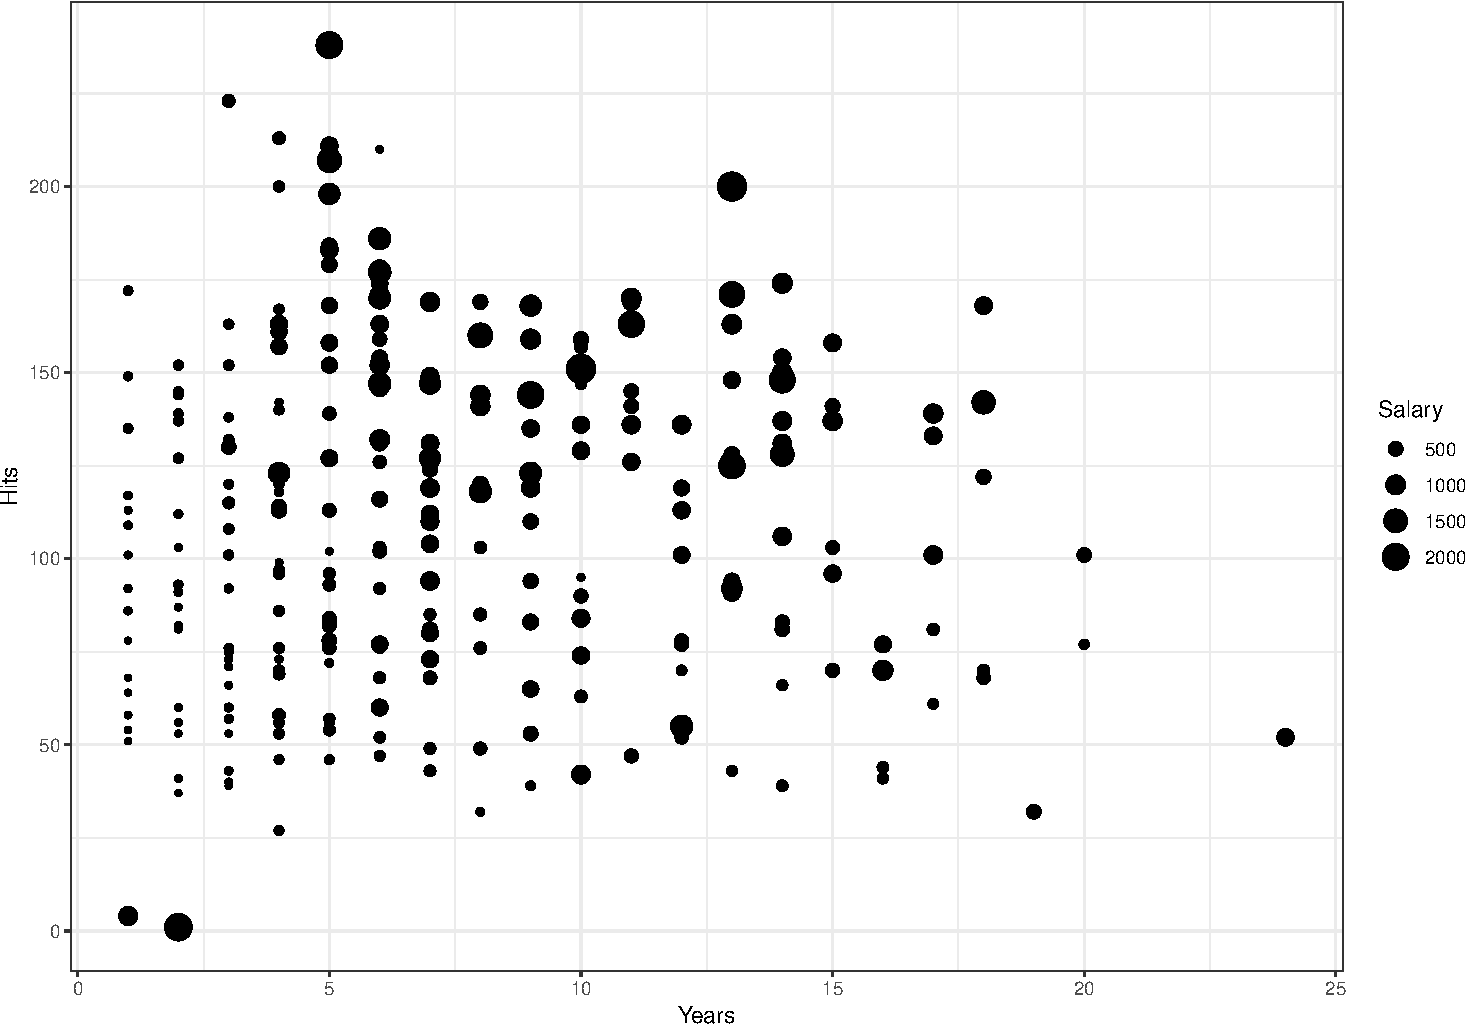
\includegraphics{week4_files/figure-beamer/unnamed-chunk-2-1.pdf}

\end{frame}

\begin{frame}{Binomial Distribution Example}

\begin{example}[Exxon]
Exxon has just bought a large tract of land in northern Quebec, with the hope of finding oil. Suppose they think that the probability that a test hole will result in oil is .2. Assume that Exxon decides to drill 7 test holes. What is the probability that
\begin{enumerate}
\item Exactly 3 of the test holes will strike oil?
\item At most 2 of the test holes will strike oil?
\item Between 3 and 5 (including 3 and 5) of the test holes will strike oil?
\item What are the mean and standard deviation of the number of test holes which strike oil.
\end{enumerate}
\end{example}

\end{frame}

\begin{frame}[fragile]{Binomial Distribution Exxon Example (\texttt{R}
code)}

\begin{Shaded}
\begin{Highlighting}[]
\CommentTok{# 1}
\KeywordTok{dbinom}\NormalTok{(}\DataTypeTok{x =} \DecValTok{3}\NormalTok{, }\DataTypeTok{size =} \DecValTok{7}\NormalTok{, }\DataTypeTok{prob =} \FloatTok{0.2}\NormalTok{)}
\end{Highlighting}
\end{Shaded}

\begin{verbatim}
## [1] 0.114688
\end{verbatim}

\begin{Shaded}
\begin{Highlighting}[]
\CommentTok{# 2}
\KeywordTok{pbinom}\NormalTok{(}\DataTypeTok{q =} \DecValTok{2}\NormalTok{, }\DataTypeTok{size =} \DecValTok{7}\NormalTok{, }\DataTypeTok{prob =} \FloatTok{0.2}\NormalTok{, }\DataTypeTok{lower.tail =} \OtherTok{TRUE}\NormalTok{)}
\end{Highlighting}
\end{Shaded}

\begin{verbatim}
## [1] 0.851968
\end{verbatim}

\begin{Shaded}
\begin{Highlighting}[]
\CommentTok{# 3}
\KeywordTok{dbinom}\NormalTok{(}\DataTypeTok{x =} \DecValTok{3}\NormalTok{, }\DataTypeTok{size =} \DecValTok{7}\NormalTok{, }\DataTypeTok{prob =} \FloatTok{0.2}\NormalTok{) }\OperatorTok{+}\StringTok{ }
\StringTok{  }\KeywordTok{dbinom}\NormalTok{(}\DataTypeTok{x =} \DecValTok{4}\NormalTok{, }\DataTypeTok{size =} \DecValTok{7}\NormalTok{, }\DataTypeTok{prob =} \FloatTok{0.2}\NormalTok{) }\OperatorTok{+}\StringTok{ }
\StringTok{  }\KeywordTok{dbinom}\NormalTok{(}\DataTypeTok{x =} \DecValTok{5}\NormalTok{, }\DataTypeTok{size =} \DecValTok{7}\NormalTok{, }\DataTypeTok{prob =} \FloatTok{0.2}\NormalTok{)}
\end{Highlighting}
\end{Shaded}

\begin{verbatim}
## [1] 0.1476608
\end{verbatim}

\end{frame}

\begin{frame}[fragile]{Binomial Distribution Exxon Example (\texttt{R}
code)}

\begin{Shaded}
\begin{Highlighting}[]
\NormalTok{(xfx <-}\StringTok{ }\KeywordTok{sapply}\NormalTok{(}\DecValTok{0}\OperatorTok{:}\DecValTok{7}\NormalTok{, }\ControlFlowTok{function}\NormalTok{(x) x }\OperatorTok{*}\StringTok{ }\KeywordTok{dbinom}\NormalTok{(}\DataTypeTok{x=}\NormalTok{x, }\DataTypeTok{size=}\DecValTok{7}\NormalTok{, }\DataTypeTok{prob=}\FloatTok{0.2}\NormalTok{))) }\CommentTok{#x*f(X=x) }
\end{Highlighting}
\end{Shaded}

\begin{verbatim}
## [1] 0.0000000 0.3670016 0.5505024 0.3440640 0.1146880 0.0215040 0.0021504
## [8] 0.0000896
\end{verbatim}

\begin{Shaded}
\begin{Highlighting}[]
\KeywordTok{sum}\NormalTok{(xfx) }\CommentTok{# E(X) or E(X) = np = 7 * 0.2 = 1.4}
\end{Highlighting}
\end{Shaded}

\begin{verbatim}
## [1] 1.4
\end{verbatim}

\begin{Shaded}
\begin{Highlighting}[]
\NormalTok{(x2fx <-}\StringTok{ }\KeywordTok{sapply}\NormalTok{(}\DecValTok{0}\OperatorTok{:}\DecValTok{7}\NormalTok{, }\ControlFlowTok{function}\NormalTok{(x) x}\OperatorTok{^}\DecValTok{2} \OperatorTok{*}\StringTok{ }\KeywordTok{dbinom}\NormalTok{(}\DataTypeTok{x=}\NormalTok{x, }\DataTypeTok{size=}\DecValTok{7}\NormalTok{, }\DataTypeTok{prob=}\FloatTok{0.2}\NormalTok{))) }\CommentTok{#x^2*f(X=x) }
\end{Highlighting}
\end{Shaded}

\begin{verbatim}
## [1] 0.0000000 0.3670016 1.1010048 1.0321920 0.4587520 0.1075200 0.0129024
## [8] 0.0006272
\end{verbatim}

\begin{Shaded}
\begin{Highlighting}[]
\KeywordTok{sum}\NormalTok{(x2fx) }\OperatorTok{-}\StringTok{ }\KeywordTok{sum}\NormalTok{(xfx)}\OperatorTok{^}\DecValTok{2} \CommentTok{# V(X)}
\end{Highlighting}
\end{Shaded}

\begin{verbatim}
## [1] 1.12
\end{verbatim}

\begin{Shaded}
\begin{Highlighting}[]
\CommentTok{# or V(X) = np(1-p) = 7 * 0.2 * 0.8 = 1.12}
\end{Highlighting}
\end{Shaded}

\end{frame}

\section{2. Bernoulli Distribution}\label{bernoulli-distribution}

\begin{frame}{Bernoulli Distribution}

The Bernoulli(\(p\)) distribution corresponds to the special case of the
\(Bin(n, p)\) distribution when \(n=1\), namely,
\[ Bern(p) \equiv Bin(1,p)\]
\[ f_X(x) = P(X=x) = p^x (1-p)^{1-x}, \quad   x = 0,1 \]

\pause

\(X_1\), \(X_2\), \ldots, \(X_n\) are chosen independently and each has
the \(Bern(p)\) distribution. Then
\[ Y= X_1+ \cdots+ X_n \sim Bin(n, p )\]

\end{frame}

\section{3. Geometric Distribution}\label{geometric-distribution}

\begin{frame}{Geometric Distribution}

Consider repeatedly flipping a coin that has probability \(p\) of coming
up heads and probability \(1-p\) of coming up tails, where
\(0 < p < 1\). Let \(X\) be the number of tails that appear before the
first head. Then for \(k\geq 0\), \(X=k\) if and only if the coin shows
exactly \(k\) tails followed by a head. The probability of this is equal
to \((1-p)^k p\)

\[f_X(k) = (1-p)^k p, \quad k = 0, 1, 2, \ldots \]

We write this as \(X\sim Geometric(p)\)

\end{frame}

\begin{frame}[fragile]{The Geometric Distribution: Geo(0.5), Geo(0.2)}

\begin{Shaded}
\begin{Highlighting}[]
\KeywordTok{plot}\NormalTok{(}\DecValTok{0}\OperatorTok{:}\DecValTok{15}\NormalTok{, }\KeywordTok{dgeom}\NormalTok{(}\DataTypeTok{x =} \DecValTok{0}\OperatorTok{:}\DecValTok{15}\NormalTok{, }\DataTypeTok{prob =} \FloatTok{0.5}\NormalTok{),}\DataTypeTok{pch =} \DecValTok{19}\NormalTok{, }\DataTypeTok{xlab=}\StringTok{"x"}\NormalTok{, }\DataTypeTok{ylab=}\StringTok{"prob"}\NormalTok{)}
\KeywordTok{points}\NormalTok{(}\DecValTok{0}\OperatorTok{:}\DecValTok{15}\NormalTok{, }\KeywordTok{dgeom}\NormalTok{(}\DecValTok{0}\OperatorTok{:}\DecValTok{15}\NormalTok{, }\DataTypeTok{prob =} \FloatTok{0.20}\NormalTok{), }\DataTypeTok{pch =} \DecValTok{19}\NormalTok{, }\DataTypeTok{col =} \StringTok{"red"}\NormalTok{)}
\KeywordTok{legend}\NormalTok{(}\StringTok{"topright"}\NormalTok{, }\KeywordTok{c}\NormalTok{(}\StringTok{"Geo(0.5)"}\NormalTok{, }\StringTok{"Geo(0.2)"}\NormalTok{), }\DataTypeTok{col =} \KeywordTok{c}\NormalTok{(}\StringTok{"black"}\NormalTok{,}\StringTok{"red"}\NormalTok{), }\DataTypeTok{pch=}\DecValTok{19}\NormalTok{)}
\end{Highlighting}
\end{Shaded}

\includegraphics{week4_files/figure-beamer/unnamed-chunk-5-1.pdf}

\end{frame}

\begin{frame}{Expected Value of Geometric Distribution}

\begin{proposition}[Expected Value Geo(p) distribution]
$X \sim Geo(p)$ then $E(X) = (1-p)/p$ and $V(X) = (1-p)/p^2$
\end{proposition}

\textbf{Proof for E(X):} \emph{on board}\\
\textbf{Proof for V(X):} \emph{exercise}

\end{frame}

\begin{frame}{Alternative form of Geometric Distribution}

Some books instead define the geometric distribution to be: \emph{the
first head requires \(k\) independent coin flips}. Let \(p\) be the
probability of a head. Then

\[f_X(k) = (1-p)^{k-1} p, \quad k = 1, 2, \ldots \]

\end{frame}

\section{4. Negative Binomial
Distribution}\label{negative-binomial-distribution}

\begin{frame}{The Negative Binomial Distribution}

\emph{A generalization of the geometric distribution}. Consider again
repeatedly flipping a coin that has probability \(p\) of coming up heads
and probability \(1-p\) of coming up tails. Let \(r\) be a positive
integer, and let \(Y\) be the number of tails that appear before the
\(r\)th head. Then for \(k \geq 0\), \(Y=k\) if and only if the coin
shows exactly \(r-1\) heads (and \(k\) tails) on the first \(r-1+k\)
flips, and then shows a head on the \((r + k)\)-th flip. The probability
of this is equal to

\pause 

\[f_{Y}(k)=\binom{r-1+k}{r-1}p^{r-1}(1-p)^{k}p = \binom{r-1+k}{k}p^{r}(1-p)^{k}, \,\,k\in 0,1,2,3,\ldots \]

\pause

The random variable \(Y\) is said to have the
Negative-Binomial\((r, p)\) distribution.

\end{frame}

\begin{frame}{The Negative Binomial Distribution}

\begin{itemize}[<+->]
\tightlist
\item
  Let \(Y\sim NegBin(r,p)\). When \(r=1\), we get then
  \(Y \sim Geo(p)\).\\
\item
  The Negative-Binomial\((r,p)\) distribution applies whenever we are
  counting the number of failures until the \(r\)th success for
  independent performances of a random system where the occurrence of
  some event is considered a success.
\end{itemize}

\end{frame}

\begin{frame}[fragile]{The Negative Binomial Distribution: NegBin(0.5),
NegBin(0.2)}

\begin{Shaded}
\begin{Highlighting}[]
\KeywordTok{plot}\NormalTok{(}\DecValTok{0}\OperatorTok{:}\DecValTok{20}\NormalTok{, }\KeywordTok{dnbinom}\NormalTok{(}\DataTypeTok{x =} \DecValTok{0}\OperatorTok{:}\DecValTok{20}\NormalTok{, }\DataTypeTok{size =} \DecValTok{2}\NormalTok{, }\DataTypeTok{prob =} \FloatTok{0.5}\NormalTok{),}\DataTypeTok{pch =} \DecValTok{19}\NormalTok{, }\DataTypeTok{xlab=}\StringTok{"x"}\NormalTok{, }\DataTypeTok{ylab=}\StringTok{"prob"}\NormalTok{)}
\KeywordTok{points}\NormalTok{(}\DecValTok{0}\OperatorTok{:}\DecValTok{20}\NormalTok{, }\KeywordTok{dnbinom}\NormalTok{(}\DecValTok{0}\OperatorTok{:}\DecValTok{20}\NormalTok{, }\DataTypeTok{size =} \DecValTok{10}\NormalTok{, }\DataTypeTok{prob =} \FloatTok{0.5}\NormalTok{), }\DataTypeTok{pch =} \DecValTok{19}\NormalTok{, }\DataTypeTok{col =} \StringTok{"red"}\NormalTok{)}
\KeywordTok{legend}\NormalTok{(}\StringTok{"topright"}\NormalTok{, }\KeywordTok{c}\NormalTok{(}\StringTok{"NB(2,0.5)"}\NormalTok{, }\StringTok{"NB(10,0.2)"}\NormalTok{), }\DataTypeTok{col =} \KeywordTok{c}\NormalTok{(}\StringTok{"black"}\NormalTok{,}\StringTok{"red"}\NormalTok{), }\DataTypeTok{pch=}\DecValTok{19}\NormalTok{)}
\end{Highlighting}
\end{Shaded}

\includegraphics{week4_files/figure-beamer/unnamed-chunk-6-1.pdf}

\end{frame}

\begin{frame}{Negative Binomial Example}

\begin{example}[Engines]
Ten percent of the engines manufactured on an assembly line are defective. If engines are randomly selected and tested, what is the probability that
\begin{enumerate}
\item the first nondefective engine will be found on the second trial?
\item the third nondefective engine will be found on the fifth trial?
\item the third nondefective engine will be found on or before the fifth trial? 
\end{enumerate}
\end{example}

\end{frame}

\section{4. The Poisson Distribution}\label{the-poisson-distribution}

\begin{frame}{The Poisson Distribution}

The binomial, geometric, and negative binomial distributions were all
derived by starting with an experiment consisting of trials or draws and
applying the laws of probability to various outcomes of the experiment.
There is no simple experiment on which the Poisson distribution is
based, although we will shortly describe how it can be obtained by
certain limiting operations.

\end{frame}

\begin{frame}{The Poisson Distribution}

We say that a random variable \(Y\) has the \(Poisson(\lambda)\)
distribution if

\[ f_Y(y) = P(Y=y) = \frac{\lambda^y}{y!}e^{-\lambda}, \quad y = 0, 1, 2, \ldots\]

\pause

Recall from calculus
\[ e^\lambda = \sum_{y=0}^{\infty} \frac{\lambda^y}{y!}\]

\pause  \emph{Exercise: show that} \(\sum_y f_Y(y) =1\)

\end{frame}

\begin{frame}[fragile]{The Poisson Distribution: Poi(2), Poi(10)}

\begin{Shaded}
\begin{Highlighting}[]
\KeywordTok{plot}\NormalTok{(}\DecValTok{0}\OperatorTok{:}\DecValTok{15}\NormalTok{, }\KeywordTok{dpois}\NormalTok{(}\DataTypeTok{x =} \DecValTok{0}\OperatorTok{:}\DecValTok{15}\NormalTok{, }\DataTypeTok{lambda =} \DecValTok{2}\NormalTok{),}\DataTypeTok{pch =} \DecValTok{19}\NormalTok{, }\DataTypeTok{xlab=}\StringTok{"x"}\NormalTok{, }\DataTypeTok{ylab=}\StringTok{"prob"}\NormalTok{)}
\KeywordTok{points}\NormalTok{(}\DecValTok{0}\OperatorTok{:}\DecValTok{15}\NormalTok{, }\KeywordTok{dpois}\NormalTok{(}\DecValTok{0}\OperatorTok{:}\DecValTok{15}\NormalTok{, }\DataTypeTok{lambda =} \DecValTok{10}\NormalTok{), }\DataTypeTok{pch =} \DecValTok{19}\NormalTok{, }\DataTypeTok{col =} \StringTok{"red"}\NormalTok{)}
\KeywordTok{legend}\NormalTok{(}\StringTok{"topright"}\NormalTok{, }\KeywordTok{c}\NormalTok{(}\StringTok{"Poi(2)"}\NormalTok{, }\StringTok{"Poi(10)"}\NormalTok{), }\DataTypeTok{col =} \KeywordTok{c}\NormalTok{(}\StringTok{"black"}\NormalTok{,}\StringTok{"red"}\NormalTok{), }\DataTypeTok{pch=}\DecValTok{19}\NormalTok{)}
\end{Highlighting}
\end{Shaded}

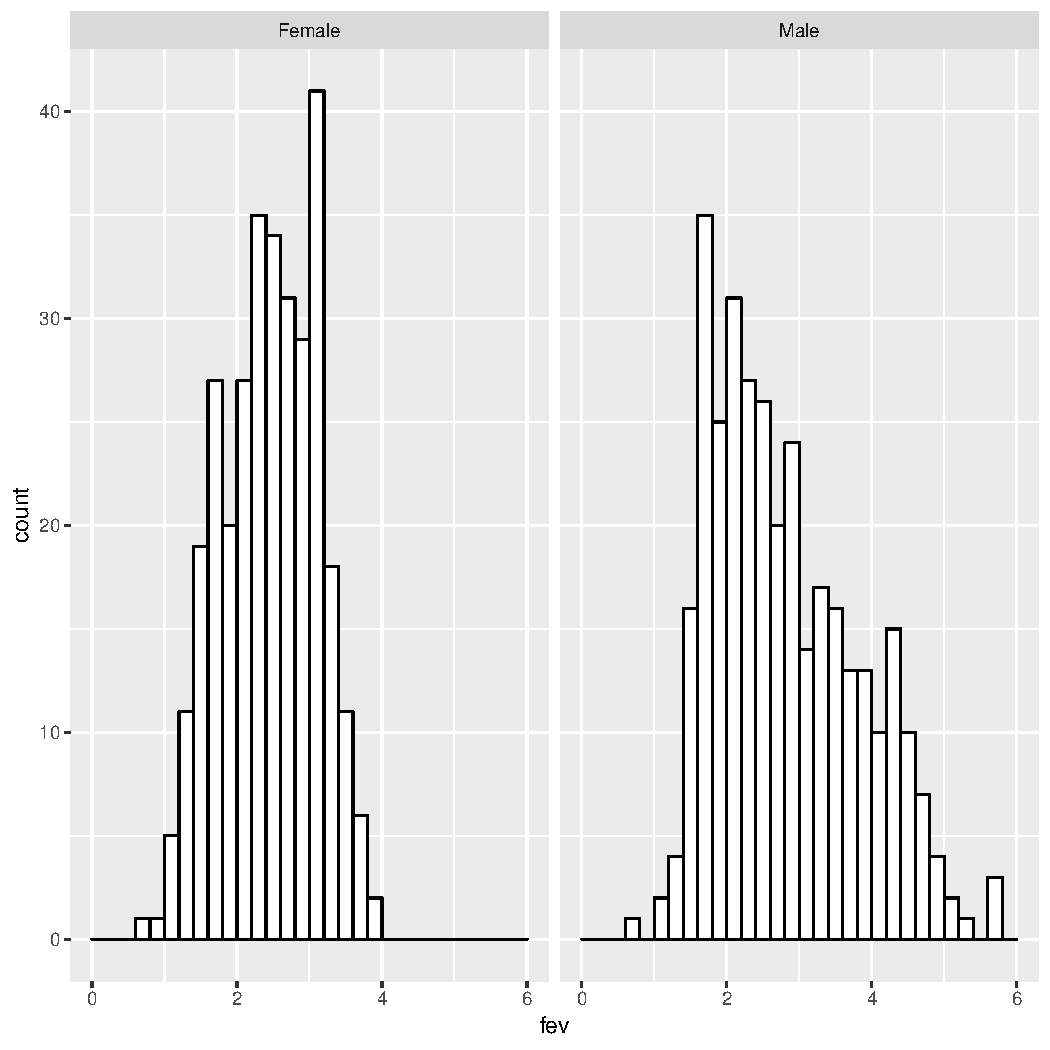
\includegraphics{week4_files/figure-beamer/unnamed-chunk-7-1.pdf}

\end{frame}

\begin{frame}{The Poisson Distribution as a Limit}

The rationale for using the Poisson distribution in many situations is
provided by the following proposition.

\begin{proposition}[Limit of a binomial is Poisson]
Suppose that $X \sim Binomial(n,p)$. If we let $p = \lambda/n$, then as $n \rightarrow \infty$, $Binomial(n,p) \rightarrow Poisson(\lambda)$. Another way of saying this: for large $n$ and small $p$, we can approximate the binomial(n,p) probability by the $Poisson(\lambda = np)$. 
\end{proposition}

\textbf{Proof:} \emph{on board}

Recall \[\left(1 + \frac{c}{n} \right)^n \rightarrow e^c\]

\end{frame}

\begin{frame}[fragile]{Poisson approximation to the Binomial}

\begin{Shaded}
\begin{Highlighting}[]
\KeywordTok{plot}\NormalTok{(}\DecValTok{0}\OperatorTok{:}\DecValTok{20}\NormalTok{, }\KeywordTok{dbinom}\NormalTok{(}\DataTypeTok{x =} \DecValTok{0}\OperatorTok{:}\DecValTok{20}\NormalTok{, }\DataTypeTok{size =} \DecValTok{100}\NormalTok{, }\DataTypeTok{p=}\FloatTok{0.1}\NormalTok{), }\DataTypeTok{pch =} \DecValTok{19}\NormalTok{, }\DataTypeTok{xlab=}\StringTok{"x"}\NormalTok{, }\DataTypeTok{ylab=}\StringTok{"prob"}\NormalTok{)}
\KeywordTok{points}\NormalTok{(}\DecValTok{0}\OperatorTok{:}\DecValTok{20}\NormalTok{, }\KeywordTok{dpois}\NormalTok{(}\DecValTok{0}\OperatorTok{:}\DecValTok{20}\NormalTok{, }\DataTypeTok{lambda =} \DecValTok{100}\OperatorTok{*}\FloatTok{0.1}\NormalTok{), }\DataTypeTok{pch =} \DecValTok{19}\NormalTok{, }\DataTypeTok{col =} \StringTok{"red"}\NormalTok{)}
\KeywordTok{legend}\NormalTok{(}\StringTok{"topright"}\NormalTok{, }\KeywordTok{c}\NormalTok{(}\StringTok{"Bin(100,0.1)"}\NormalTok{, }\StringTok{"Poi(10)"}\NormalTok{), }\DataTypeTok{col =} \KeywordTok{c}\NormalTok{(}\StringTok{"black"}\NormalTok{,}\StringTok{"red"}\NormalTok{), }\DataTypeTok{pch=}\DecValTok{19}\NormalTok{)}
\end{Highlighting}
\end{Shaded}

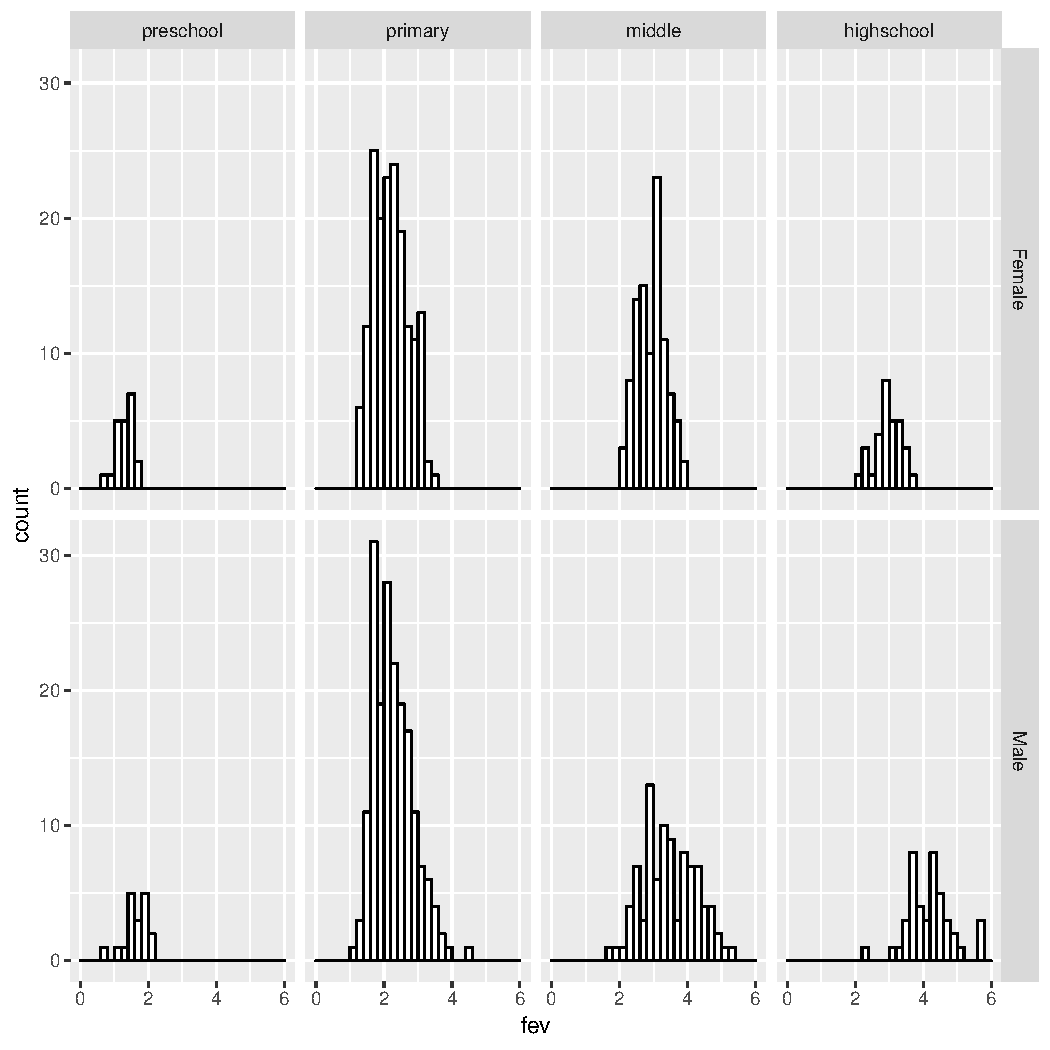
\includegraphics{week4_files/figure-beamer/unnamed-chunk-8-1.pdf}

\end{frame}

\begin{frame}{Poisson Expectation and Variance}

Let \(X \sim Poisson(\lambda)\), then
\[E(X) = \lambda, \quad V(X) = \lambda\]

recall: \[e^\lambda = \sum_{x=0}^{\infty} \frac{\lambda^x}{x!} \]

\textbf{Proof:} \emph{on board}

\end{frame}

\begin{frame}{Summary of Discrete Distributions}

\footnotesize{
\begin{tabular}{ll}
Single 0-1 trial - count number of 1s & $\Longrightarrow $ BERNOULLI
DISTRIBUTION \\
&  \\
$n$ independent 0-1 trials - count number of 1s & $\Longrightarrow $
BINOMIAL DISTRIBUTION \\
&  \\
Sequence of independent 0-1 trials & $\Longrightarrow $ GEOMETRIC
DISTRIBUTION \\
- count number of trials until first 1 &  \\
&  \\
Sequence of independent 0-1 trials - & $\Longrightarrow $ NEGATIVE BINOMIAL
DISTRIBUTION \\
count number of trials until $r^{th}$ 1 is observed &  \\
&  \\
Limiting case of binomial distribution & $\Longrightarrow $ POISSON
DISTRIBUTION
\end{tabular}
}

\end{frame}

\section{Moment Generating Functions}\label{moment-generating-functions}

\begin{frame}{Moment Generating Functions (MGFs)}

\begin{definition}[Moments]
Let $X$ be a random variable and $k$ an integer with $k \geq 0$. Suppose that $E(|X^k|) < \infty$ (i.e. the expected value exists). Then the number $\mu_k^\prime = E(X^k)$ is called the $k$th moment of $X$ about the origin. The number $\mu_k = E[(X-\mu)^k ]$ (where $\mu = \mu_1^\prime = E(X)$) is called the $k$th moment of $X$ about its mean.
\end{definition}

\end{frame}

\begin{frame}{Moment Generating Functions (MGFs)}

\begin{definition}[MGFs]
Let $X$ be a random variable. If there exists a $\delta >0$, such that $E(e^{tX}) < \infty$ for all $-\delta < t < \delta$, then
\[M_X(t) \equiv E(e^{tX}), \quad -\delta < t < \delta\]
is called the MGF of $X$. For a discrete RV we have
\pause
\[M_X(t) = \sum_{x \in R_X} e^{tx} f_X(x)\]
\end{definition}

\end{frame}

\begin{frame}{MGF Examples}

\begin{example}[Constant]
If $X=c$, then \[M_X(t) = E(e^{tc}) = e^{tc}\]

\end{example}

\end{frame}

\begin{frame}{MGF Examples}

\begin{example}[Binomial]
If $X\sim Binomial(n, p)$, then \[M_X(t) = E(e^{tx}) = \sum_{x=0}^{n}e^{tx} \binom{n}{x} p^x (1-p)^{n-x} = (pe^t + (1-p))^n\]



\end{example}

\textbf{Proof:} \emph{on board}

\end{frame}

\begin{frame}{MGF Examples}

\begin{example}[Poisson]
If $X\sim Poisson(\lambda)$, then \[M_X(t) = e^{-\lambda(1-e^t)} \]

\end{example}

\textbf{Proof:} \emph{on board}

\end{frame}

\begin{frame}{Why should we care about MGFs}

\begin{proposition}
\[M_X^{(n)}(0) = E(X^n), \quad n=0,1,\ldots\]
In words, the $n^{th}$ derivative of the MGF evaluated at $t=0$ is the $n^{th}$ moment of $X$
\end{proposition}

\end{frame}

\begin{frame}{Why should we care about MGFs}

\begin{proof}
$M_X^{(n)}(0) = E(e^0) = E(1) =1$. Then
\begin{align*}
M_X^\prime (t) &= \sum_{x \in R_X} x e^{tx} f_X(x) \\
M_X^{\prime\prime} (t) &= \sum_{x \in R_X} x^2 e^{tx} f_X(x) \\
\vdots & = \vdots \\
M_X^{(n)} (t) &= \sum_{x \in R_X} x^n e^{tx} f_X(x) 
\end{align*}
From which $M_X^\prime (0) = E(X), M_X^{\prime\prime}(0) = E(X^2)$, and so on.
\end{proof}

\end{frame}

\begin{frame}{Examples of Moments using MGFs}

\begin{example}[Binomial]
If $X\sim Binomial(n,p)$, then 
\begin{align*}
M_X^{\prime}(t) &= \frac{d}{dt} (pe^t + (1-p))^n \\
& = n(pe^t + (1-p))^{n-1} (pe^t)\\
M_X^{\prime\prime}(t) &= n(pe^t + (1-p))^{n-1}pe^t + n(n-1)(pe^t + (1-p))^{n-2}(pe^t)^2
\end{align*}
So $E(X) = M_X^\prime(0) = np$ and $E(X^2) = M_X^{\prime\prime}(0) = np + n(n-1)p^2$ and $V(X) = np + n(n-1)p^2 - n^2p^2 = np(1-p)$
\end{example}

\end{frame}

\end{document}
